\documentclass[10pt,a4paper]{article}
\usepackage[margin=18mm,top=22mm,bottom=18mm,headsep=7mm,footskip=9mm]{geometry}
\usepackage{fontspec,amsmath,amssymb,array,tabularx,xcolor,colortbl,tikz,fancyhdr,hyperref}
\usetikzlibrary{arrows.meta}
\setmainfont{NotoSansKR-Regular.ttf}[Path=../../../common/assets/fonts/,BoldFont=NotoSansKR-Semibold.ttf]
\newfontfamily\brandfont{NotoSansKR-Regular.ttf}[Path=../../../common/assets/fonts/,BoldFont=NotoSansKR-Semibold.ttf]
\definecolor{ink}{HTML}{25343D}
\definecolor{accent}{HTML}{216B7A}
\definecolor{muted}{HTML}{637078}
\definecolor{grid}{HTML}{D2DCDF}
\definecolor{soft}{HTML}{F2F6F6}
\definecolor{vectorblue}{HTML}{266CA8}
\definecolor{answerred}{HTML}{C42030}
\newif\ifanswers\answersfalse
\hypersetup{colorlinks=true,urlcolor=accent,pdftitle={OZ Lab AI Study: Multiple Linear Regression and Feature Scaling},pdfauthor={OZ Lab}}
\setlength{\parindent}{0pt}\setlength{\parskip}{2pt}\setlength{\headheight}{21pt}
\setlength{\tabcolsep}{4pt}\renewcommand{\arraystretch}{1.1}\arrayrulecolor{grid}
\pagestyle{fancy}\fancyhf{}
\fancyhead[L]{\brandfont\fontsize{8}{10}\selectfont\bfseries\color{ink}OZ Lab\quad AI Study}
\fancyhead[R]{\brandfont\fontsize{7}{10}\selectfont\color{muted}Multiple Linear Regression / Feature Scaling}
\fancyfoot[L]{\brandfont\fontsize{7}{9}\selectfont\color{muted}C1 W2\quad /\quad SLIDES 83 TO 99}
\fancyfoot[R]{\brandfont\fontsize{8}{10}\selectfont\color{ink}0\thepage\quad{\color{muted}/\ 08}}
\renewcommand{\headrulewidth}{.3pt}
\renewcommand{\headrule}{\hbox to\headwidth{\color{grid}\leaders\hrule height\headrulewidth\hfill}}
\newcommand{\sect}[2]{\par\vspace{2mm}{\brandfont\fontsize{10}{15}\selectfont\bfseries\color{accent}#1}\quad{\fontsize{14}{19}\selectfont\bfseries\color{ink}#2}\par\vspace{3mm}}
\newcommand{\q}[2]{\par\vspace{3mm}\noindent\makebox[7mm][l]{\brandfont\fontsize{9}{14}\selectfont\bfseries\color{accent}#1}\begin{minipage}[t]{\dimexpr\linewidth-7mm}\fontsize{9.3}{14}\selectfont #2\end{minipage}\par\vspace{1mm}}
\newcommand{\note}[1]{\par\hspace*{7mm}\begin{minipage}{\dimexpr\linewidth-7mm}\fontsize{7.5}{10.5}\selectfont\color{muted}* #1\end{minipage}\par}
\newcommand{\formula}[1]{\par\vspace{1mm}\begingroup\setlength{\fboxsep}{2.3mm}\colorbox{soft}{\begin{minipage}{\dimexpr\linewidth-4.6mm}\fontsize{10}{15}\selectfont$\displaystyle #1$\end{minipage}}\endgroup\par\vspace{1mm}}
\newcommand{\given}[1]{\par\vspace{2mm}\hspace*{7mm}{\fontsize{9.3}{14}\selectfont$\displaystyle #1$}\par\vspace{1mm}}
\newcommand{\ansblank}[2]{\makebox[#1]{\strut\ifanswers\smash{\textcolor{answerred}{\ensuremath{#2}}}\else\textcolor{grid}{\rule{#1}{.3pt}}\fi}}
\newcommand{\cellanswer}[1]{\smash{\makebox[0pt]{\ifanswers\textcolor{answerred}{$#1$}\fi}}}
\newcommand{\tablerow}{\rule[-1.8mm]{0pt}{7mm}}
\newcommand{\solution}[2]{\par\vspace{1.5mm}\begin{minipage}[t][#1][t]{\linewidth}\vspace{0pt}\fontsize{8}{11}\selectfont\ifanswers\leavevmode\color{answerred}#2\else{\color{grid}\hrule height .3pt}\fi\end{minipage}\par}
\newcommand{\pick}[3]{{\leavevmode\ifanswers\ifnum#1=#2\color{answerred}\fi\fi$\square$\ #3}}
\newcommand{\choices}[3]{\par\vspace{1.5mm}\hspace*{7mm}{\fontsize{8.5}{13}\selectfont\pick{1}{#3}{#1}\qquad\pick{2}{#3}{#2}}\par\vspace{1mm}}
\AtBeginDocument{\fontsize{9.3}{14}\selectfont\color{ink}}
\begin{document}
{\brandfont\fontsize{18}{23}\selectfont\bfseries Multiple Linear Regression\par}
\vspace{1mm}{\fontsize{10.5}{15}\selectfont Multiple inputs and comparable feature scales}\hfill{\ifanswers\color{answerred}\bfseries Worked answers\else\color{muted}Hand-calculation worksheet\fi}\par
\vspace{3mm}{\fontsize{8}{12}\selectfont\color{muted}Name\quad\rule{33mm}{.3pt}\hfill Date\quad\rule{28mm}{.3pt}}\par
\sect{01}{Data and Features}
\note{Synthetic practice data\quad Area is entered in units of 10\,$\mathrm{m}^2$ · For 120\,$\mathrm{m}^2$, use $x_1=12$}
\begingroup\fontsize{8.3}{11}\selectfont
\begin{tabularx}{\linewidth}{@{}c*{4}{>{\centering\arraybackslash}X}@{}}
\rowcolor{soft}\tablerow House $i$ & Area ($\mathrm{m}^2$) & Input $x_1$ & Rooms $x_2$ & Target $y$ (10M KRW)\\\hline
\rule[-1.8mm]{0pt}{7mm} $1$ & $120$ & $12$ & $3$ & $21$\\\hline
\rule[-1.8mm]{0pt}{7mm} $2$ & $60$ & $6$ & $2$ & $12$\\\hline
\rule[-1.8mm]{0pt}{7mm} $3$ & $160$ & $16$ & $4$ & $28$\\\hline
\rule[-1.8mm]{0pt}{7mm} $4$ & $100$ & $10$ & $3$ & $22$\\\hline
\rule[-1.8mm]{0pt}{7mm} $5$ & $180$ & $18$ & $4$ & $31$\\\hline
\rule[-1.8mm]{0pt}{7mm} $6$ & $80$ & $8$ & $2$ & $15$\\\hline
\rule[-1.8mm]{0pt}{7mm} $7$ & $140$ & $14$ & $3$ & $25$\\\hline
\end{tabularx}\endgroup\par
\q{1}{Write the number of examples $m$ and features $n$}
\given{m=\ansblank{16mm}{7}\qquad n=\ansblank{16mm}{2}}
\q{2}{Express the input of House 4 as a vector and find the following values}
\formula{\mathbf{x}^{(i)}=[x_1^{(i)},x_2^{(i)}]\qquad i=\text{house index},\quad j=\text{feature index}}
\given{\mathbf{x}^{(4)}=[\ansblank{12mm}{10},\ansblank{12mm}{3}]\qquad x_2^{(4)}=\ansblank{12mm}{3}\qquad y^{(4)}=\ansblank{12mm}{22}}
\q{3}{Is a larger house always more expensive in the actual data? Compare Houses 1 and 4}
\begin{center}
\begin{tikzpicture}[x=.94cm,y=.165cm]
\path[use as bounding box] (4.2,7) rectangle (20.1,37);
\draw[grid,line width=.22pt,xstep=2,ystep=5] (5,10) grid (19,35);
\draw[-{Stealth[length=1.7mm]},ink,line width=.5pt] (5,10)--(19.6,10) node[right]{\scriptsize$x_1$};
\draw[-{Stealth[length=1.7mm]},ink,line width=.5pt] (5,10)--(5,36) node[above]{\scriptsize$y$};
\node[below,fill=white,inner sep=.7pt] at (6,10){\scriptsize$6$};
\node[below,fill=white,inner sep=.7pt] at (8,10){\scriptsize$8$};
\node[below,fill=white,inner sep=.7pt] at (10,10){\scriptsize$10$};
\node[below,fill=white,inner sep=.7pt] at (12,10){\scriptsize$12$};
\node[below,fill=white,inner sep=.7pt] at (14,10){\scriptsize$14$};
\node[below,fill=white,inner sep=.7pt] at (16,10){\scriptsize$16$};
\node[below,fill=white,inner sep=.7pt] at (18,10){\scriptsize$18$};
\node[left,fill=white,inner sep=.7pt] at (5,10){\scriptsize$10$};
\node[left,fill=white,inner sep=.7pt] at (5,15){\scriptsize$15$};
\node[left,fill=white,inner sep=.7pt] at (5,20){\scriptsize$20$};
\node[left,fill=white,inner sep=.7pt] at (5,25){\scriptsize$25$};
\node[left,fill=white,inner sep=.7pt] at (5,30){\scriptsize$30$};
\node[left,fill=white,inner sep=.7pt] at (5,35){\scriptsize$35$};
\fill[vectorblue] (12,21) circle(1.9pt);
\node[vectorblue,above right,fill=white,inner sep=.6pt] at (12,21){\scriptsize$1$};
\fill[vectorblue] (6,12) circle(1.9pt);
\node[vectorblue,above right,fill=white,inner sep=.6pt] at (6,12){\scriptsize$2$};
\fill[vectorblue] (16,28) circle(1.9pt);
\node[vectorblue,above right,fill=white,inner sep=.6pt] at (16,28){\scriptsize$3$};
\fill[vectorblue] (10,22) circle(1.9pt);
\node[vectorblue,above left,fill=white,inner sep=.6pt] at (10,22){\scriptsize$4$};
\fill[vectorblue] (18,31) circle(1.9pt);
\node[vectorblue,above right,fill=white,inner sep=.6pt] at (18,31){\scriptsize$5$};
\fill[vectorblue] (8,15) circle(1.9pt);
\node[vectorblue,above right,fill=white,inner sep=.6pt] at (8,15){\scriptsize$6$};
\fill[vectorblue] (14,25) circle(1.9pt);
\node[vectorblue,above right,fill=white,inner sep=.6pt] at (14,25){\scriptsize$7$};
\end{tikzpicture}
\end{center}
\choices{Always more expensive}{Not always}{2}
\solution{11mm}{House 4: 100\,$\mathrm{m}^2$, KRW 220 million\quad House 1: 120\,$\mathrm{m}^2$, KRW 210 million\\Larger houses tend to cost more, but area alone cannot explain every price difference}
\vfill{\fontsize{6.8}{10}\selectfont\color{muted}Reference · DeepLearning.AI / Stanford Online · Machine Learning Specialization · Current lesson slides 83 to 99}

\newpage\sect{02}{Prediction and Cost}
\formula{f_{\mathbf w,b}(\mathbf x)=w_1x_1+w_2x_2+b\qquad \mathbf w=[1,3],\quad b=2}
\q{4}{Calculate the price of House 4 using both the expanded expression and a dot product}
\formula{\mathbf w\cdot\mathbf x=w_1x_1+w_2x_2\qquad f_{\mathbf w,b}(\mathbf x)=\mathbf w\cdot\mathbf x+b}
\given{1\times10+3\times3+2=\ansblank{27mm}{10+9+2=21}}
\given{[1,3]\cdot[10,3]+2=\ansblank{27mm}{19+2=21}}
\solution{8mm}{A dot product multiplies matching entries and adds the products\quad Add $b$ once at the end\\Two inputs still produce one predicted price}
\q{5}{Calculate each of the seven predictions, errors, and squared errors}
\formula{\hat y^{(i)}=x_1^{(i)}+3x_2^{(i)}+2\qquad e^{(i)}=\hat y^{(i)}-y^{(i)}}
\begingroup\fontsize{8.3}{11}\selectfont
\begin{tabularx}{\linewidth}{@{}c c c *{3}{>{\centering\arraybackslash}X}@{}}
\rowcolor{soft}\tablerow House & Prediction expression & $y^{(i)}$ & $\hat y^{(i)}$ & $e^{(i)}$ & $(e^{(i)})^2$\\\hline
\rule[-1.8mm]{0pt}{9mm} $1$ & $12+3\times3+2$ & $21$ & \cellanswer{12+9+2=23} & \cellanswer{23-21=2} & \cellanswer{(2)^2=4}\\\hline
\rule[-1.8mm]{0pt}{9mm} $2$ & $6+3\times2+2$ & $12$ & \cellanswer{6+6+2=14} & \cellanswer{14-12=2} & \cellanswer{(2)^2=4}\\\hline
\rule[-1.8mm]{0pt}{9mm} $3$ & $16+3\times4+2$ & $28$ & \cellanswer{16+12+2=30} & \cellanswer{30-28=2} & \cellanswer{(2)^2=4}\\\hline
\rule[-1.8mm]{0pt}{9mm} $4$ & $10+3\times3+2$ & $22$ & \cellanswer{10+9+2=21} & \cellanswer{21-22=-1} & \cellanswer{(-1)^2=1}\\\hline
\rule[-1.8mm]{0pt}{9mm} $5$ & $18+3\times4+2$ & $31$ & \cellanswer{18+12+2=32} & \cellanswer{32-31=1} & \cellanswer{(1)^2=1}\\\hline
\rule[-1.8mm]{0pt}{9mm} $6$ & $8+3\times2+2$ & $15$ & \cellanswer{8+6+2=16} & \cellanswer{16-15=1} & \cellanswer{(1)^2=1}\\\hline
\rule[-1.8mm]{0pt}{9mm} $7$ & $14+3\times3+2$ & $25$ & \cellanswer{14+9+2=25} & \cellanswer{25-25=0} & \cellanswer{(0)^2=0}\\\hline
\end{tabularx}\endgroup\par
\q{6}{Calculate the MSE and cost}
\formula{\mathrm{MSE}=\frac1m\sum_{i=1}^m(e^{(i)})^2\qquad J(\mathbf w,b)=\frac1{2m}\sum_{i=1}^m(e^{(i)})^2=\frac12\mathrm{MSE}}
\given{\sum_{i=1}^{7}(e^{(i)})^2=\ansblank{70mm}{4+4+4+1+1+1+0=15}}
\given{\mathrm{MSE}=\ansblank{22mm}{\frac{15}{7}}\qquad J(\mathbf w,b)=\ansblank{22mm}{\frac{15}{14}}}
\solution{11mm}{$\mathrm{MSE}=15\div7=\frac{15}{7}$\quad $J=15\div(2\times7)=\frac{15}{14}\approx1.071$\\$m$ counts houses\quad Even with two features, divide by $2m=14$}

\newpage\sect{03}{Prediction Plot}
\q{7}{Use each house\textquotesingle s area and room count to plot \textbf{the predictions from Question 5}\\[1mm]Draw circles, then connect each prediction to the same house\textquotesingle s actual price with a \textbf{vertical line}}
\formula{P_i=(x_1^{(i)},\hat y^{(i)})\qquad \hat y^{(i)}=x_1^{(i)}+3x_2^{(i)}+2}
\begingroup\fontsize{8.3}{11}\selectfont
\begin{tabularx}{\linewidth}{@{}*{7}{>{\centering\arraybackslash}X}@{}}
\rowcolor{soft}\tablerow $i=1$ & $i=2$ & $i=3$ & $i=4$ & $i=5$ & $i=6$ & $i=7$\\\hline
\rule[-1.8mm]{0pt}{10mm} \cellanswer{(12,23)} & \cellanswer{(6,14)} & \cellanswer{(16,30)} & \cellanswer{(10,21)} & \cellanswer{(18,32)} & \cellanswer{(8,16)} & \cellanswer{(14,25)}\\\hline
\end{tabularx}\endgroup\par
\vspace{5mm}\note{Same axes and actual data as Question 3\quad Blue points: actual prices · Circles: predictions}
\begin{center}
\begin{tikzpicture}[x=.94cm,y=.165cm]
\path[use as bounding box] (4.2,7) rectangle (20.1,37);
\draw[grid,line width=.22pt,xstep=2,ystep=5] (5,10) grid (19,35);
\draw[-{Stealth[length=1.7mm]},ink,line width=.5pt] (5,10)--(19.6,10) node[right]{\scriptsize$x_1$};
\draw[-{Stealth[length=1.7mm]},ink,line width=.5pt] (5,10)--(5,36) node[above]{\scriptsize$y$};
\node[below,fill=white,inner sep=.7pt] at (6,10){\scriptsize$6$};
\node[below,fill=white,inner sep=.7pt] at (8,10){\scriptsize$8$};
\node[below,fill=white,inner sep=.7pt] at (10,10){\scriptsize$10$};
\node[below,fill=white,inner sep=.7pt] at (12,10){\scriptsize$12$};
\node[below,fill=white,inner sep=.7pt] at (14,10){\scriptsize$14$};
\node[below,fill=white,inner sep=.7pt] at (16,10){\scriptsize$16$};
\node[below,fill=white,inner sep=.7pt] at (18,10){\scriptsize$18$};
\node[left,fill=white,inner sep=.7pt] at (5,10){\scriptsize$10$};
\node[left,fill=white,inner sep=.7pt] at (5,15){\scriptsize$15$};
\node[left,fill=white,inner sep=.7pt] at (5,20){\scriptsize$20$};
\node[left,fill=white,inner sep=.7pt] at (5,25){\scriptsize$25$};
\node[left,fill=white,inner sep=.7pt] at (5,30){\scriptsize$30$};
\node[left,fill=white,inner sep=.7pt] at (5,35){\scriptsize$35$};
\ifanswers
\draw[answerred,line width=.55pt] (12,21)--(12,23);
\draw[answerred,line width=.55pt] (6,12)--(6,14);
\draw[answerred,line width=.55pt] (16,28)--(16,30);
\draw[answerred,line width=.55pt] (10,22)--(10,21);
\draw[answerred,line width=.55pt] (18,31)--(18,32);
\draw[answerred,line width=.55pt] (8,15)--(8,16);
\fi
\fill[vectorblue] (12,21) circle(1.9pt);
\node[vectorblue,below right,fill=white,inner sep=.6pt] at (12,21){\scriptsize$1$};
\fill[vectorblue] (6,12) circle(1.9pt);
\node[vectorblue,below right,fill=white,inner sep=.6pt] at (6,12){\scriptsize$2$};
\fill[vectorblue] (16,28) circle(1.9pt);
\node[vectorblue,below right,fill=white,inner sep=.6pt] at (16,28){\scriptsize$3$};
\fill[vectorblue] (10,22) circle(1.9pt);
\node[vectorblue,above left,fill=white,inner sep=.6pt] at (10,22){\scriptsize$4$};
\fill[vectorblue] (18,31) circle(1.9pt);
\node[vectorblue,below right,fill=white,inner sep=.6pt] at (18,31){\scriptsize$5$};
\fill[vectorblue] (8,15) circle(1.9pt);
\node[vectorblue,below right,fill=white,inner sep=.6pt] at (8,15){\scriptsize$6$};
\fill[vectorblue] (14,25) circle(1.9pt);
\node[vectorblue,above right,fill=white,inner sep=.6pt] at (14,25){\scriptsize$7$};
\ifanswers
\draw[answerred,line width=.65pt] (12,23) circle(2.5pt);
\draw[answerred,line width=.65pt] (6,14) circle(2.5pt);
\draw[answerred,line width=.65pt] (16,30) circle(2.5pt);
\draw[answerred,line width=.65pt] (10,21) circle(2.5pt);
\draw[answerred,line width=.65pt] (18,32) circle(2.5pt);
\draw[answerred,line width=.65pt] (8,16) circle(2.5pt);
\draw[answerred,line width=.65pt] (14,25) circle(2.5pt);
\fi
\end{tikzpicture}
\end{center}
\vspace{4mm}Use the plot to check the error signs for Houses 1 and 4\par
\formula{e^{(i)}=\hat y^{(i)}-y^{(i)}\qquad \text{vertical distance}=|e^{(i)}|}
\given{e^{(1)}=\ansblank{32mm}{23-21=2}\qquad e^{(4)}=\ansblank{32mm}{21-22=-1}}
\solution{17mm}{House 1: prediction is 2 above the actual price; its circle is above the blue point\\House 4: prediction is 1 below the actual price; its circle is below the blue point\\House 7: $25-25=0$, so the points overlap\\A longer vertical line means a larger error magnitude; the cost uses its square}

\newpage\sect{04}{Parameter Update}
\formula{\mathbf w=[1,3],\quad b=2\qquad \alpha=0.01\qquad m=7}
\q{8}{Copy the errors from Question 5 and multiply each by the corresponding feature}
\formula{e^{(i)}=f_{\mathbf w,b}(\mathbf x^{(i)})-y^{(i)}\qquad e^{(i)}x_1^{(i)},\quad e^{(i)}x_2^{(i)}}
\begingroup\fontsize{8.3}{11}\selectfont
\begin{tabularx}{\linewidth}{@{}c*{3}{>{\centering\arraybackslash}X}@{}}
\rowcolor{soft}\tablerow House & $e^{(i)}$ & $e^{(i)}x_1^{(i)}$ & $e^{(i)}x_2^{(i)}$\\\hline
\rule[-1.8mm]{0pt}{8mm} $1$ & \cellanswer{2} & \cellanswer{2\times12=24} & \cellanswer{2\times3=6}\\\hline
\rule[-1.8mm]{0pt}{8mm} $2$ & \cellanswer{2} & \cellanswer{2\times6=12} & \cellanswer{2\times2=4}\\\hline
\rule[-1.8mm]{0pt}{8mm} $3$ & \cellanswer{2} & \cellanswer{2\times16=32} & \cellanswer{2\times4=8}\\\hline
\rule[-1.8mm]{0pt}{8mm} $4$ & \cellanswer{-1} & \cellanswer{-1\times10=-10} & \cellanswer{-1\times3=-3}\\\hline
\rule[-1.8mm]{0pt}{8mm} $5$ & \cellanswer{1} & \cellanswer{1\times18=18} & \cellanswer{1\times4=4}\\\hline
\rule[-1.8mm]{0pt}{8mm} $6$ & \cellanswer{1} & \cellanswer{1\times8=8} & \cellanswer{1\times2=2}\\\hline
\rule[-1.8mm]{0pt}{8mm} $7$ & \cellanswer{0} & \cellanswer{0\times14=0} & \cellanswer{0\times3=0}\\\hline
\rule[-1.8mm]{0pt}{8mm} Sum & \cellanswer{7} & \cellanswer{84} & \cellanswer{21}\\\hline
\end{tabularx}\endgroup\par
\q{9}{Calculate the gradient for each parameter}
\formula{g_1=\frac{\partial J}{\partial w_1}=\frac1m\sum_{i=1}^m e^{(i)}x_1^{(i)}\quad g_2=\frac{\partial J}{\partial w_2}=\frac1m\sum_{i=1}^m e^{(i)}x_2^{(i)}\quad g_b=\frac{\partial J}{\partial b}=\frac1m\sum_{i=1}^m e^{(i)}}
\given{g_1=\ansblank{25mm}{\frac{84}{7}=12}\qquad g_2=\ansblank{25mm}{\frac{21}{7}=3}\qquad g_b=\ansblank{25mm}{\frac{7}{7}=1}}
\note{Use the provided derivatives\quad The gradient for $b$ has no feature multiplier}
\q{10}{Update all three values simultaneously from the same starting point}
\formula{w_1^{\rm new}=w_1-\alpha g_1\qquad w_2^{\rm new}=w_2-\alpha g_2\qquad b^{\rm new}=b-\alpha g_b}
\given{w_1^{\rm new}=1-0.01\times\ansblank{12mm}{12}=\ansblank{17mm}{0.88}}
\given{w_2^{\rm new}=3-0.01\times\ansblank{12mm}{3}=\ansblank{17mm}{2.97}\qquad b^{\rm new}=2-0.01\times\ansblank{12mm}{1}=\ansblank{17mm}{1.99}}
\solution{10mm}{$0.01\times12=0.12$, so $w_1^{\rm new}=1-0.12=0.88$\\$w_2^{\rm new}=3-0.03=2.97$\quad $b^{\rm new}=2-0.01=1.99$}
\q{11}{Can you update $w_1$ first, then use its new value to recalculate $g_2$?}
\choices{Yes}{No}{2}
\solution{8mm}{Calculate $g_1,g_2,g_b$ using the same pre-update $\mathbf w=[1,3],b=2$\\Use the same seven errors, then apply all new parameter values together}

\newpage\sect{05}{Cost and Feature Scale}
\q{12}{Calculate House 4\textquotesingle s error after the update and compare it with the overall cost change}
\formula{f_{\rm new}(\mathbf x)=0.88x_1+2.97x_2+1.99\qquad \mathbf x^{(4)}=[10,3],\quad y^{(4)}=22}
\given{\hat y_{\rm new}^{(4)}=\ansblank{40mm}{8.8+8.91+1.99=19.70}\qquad e_{\rm new}^{(4)}=\ansblank{28mm}{19.70-22=-2.30}}
\note{Overall cost across all seven houses: $J_{\rm old}=15/14\approx1.071$, $J_{\rm new}=11.8016/14\approx0.843$}
\choices{Lower cost means every error decreases}{Some errors can increase}{2}
\solution{10mm}{House 4\textquotesingle s error magnitude grows from $|21-22|=1$ to $|19.70-22|=2.30$\\Overall $J$ drops from about $1.071$ to $0.843$: it evaluates all seven errors together}
\q{13}{For House 1, compare prediction changes when each weight is increased by $0.1$ separately}
\formula{\Delta\hat y=x_j\Delta w_j\qquad \mathbf x^{(1)}=[12,3]\quad (\text{other values fixed})}
\given{\Delta w_1=0.1\ \Rightarrow\ \Delta\hat y=\ansblank{27mm}{12\times0.1=1.2}\qquad \Delta w_2=0.1\ \Rightarrow\ \Delta\hat y=\ansblank{27mm}{3\times0.1=0.3}}
\solution{9mm}{The same $0.1$ weight change gives a larger prediction change for area\\Weight magnitude alone does not establish feature importance; input units and scale also matter}
\q{14}{The contours of our cost function are shown below\\[1mm]Analyze any features that could make it difficult for gradient descent to reach the minimum}
\note{Same seven examples, $J(w_1,w_2,b=2)$\quad A slice at fixed $b=2$ · Blue point: minimum of this slice}
\begin{center}
\begin{tikzpicture}[x=1cm,y=1cm]
\path[use as bounding box] (-.65,-.4) rectangle (7.4,7.1);
\draw[grid,line width=.22pt] (0.0,0)--(0.0,6.6);
\node[below,fill=white,inner sep=.7pt] at (0.0,1.6499999999999997){\scriptsize$-4$};
\draw[grid,line width=.22pt] (1.0999999999999999,0)--(1.0999999999999999,6.6);
\node[below,fill=white,inner sep=.7pt] at (1.0999999999999999,1.6499999999999997){\scriptsize$-2$};
\draw[grid,line width=.22pt] (2.1999999999999997,0)--(2.1999999999999997,6.6);
\node[below,fill=white,inner sep=.7pt] at (2.1999999999999997,1.6499999999999997){\scriptsize$0$};
\draw[grid,line width=.22pt] (3.2999999999999994,0)--(3.2999999999999994,6.6);
\node[below,fill=white,inner sep=.7pt] at (3.2999999999999994,1.6499999999999997){\scriptsize$2$};
\draw[grid,line width=.22pt] (4.3999999999999995,0)--(4.3999999999999995,6.6);
\node[below,fill=white,inner sep=.7pt] at (4.3999999999999995,1.6499999999999997){\scriptsize$4$};
\draw[grid,line width=.22pt] (5.5,0)--(5.5,6.6);
\node[below,fill=white,inner sep=.7pt] at (5.5,1.6499999999999997){\scriptsize$6$};
\draw[grid,line width=.22pt] (6.599999999999999,0)--(6.599999999999999,6.6);
\node[below,fill=white,inner sep=.7pt] at (6.599999999999999,1.6499999999999997){\scriptsize$8$};
\draw[grid,line width=.22pt] (0,0.5499999999999999)--(6.6,0.5499999999999999);
\node[left,fill=white,inner sep=.7pt] at (2.1999999999999997,0.5499999999999999){\scriptsize$-2$};
\draw[grid,line width=.22pt] (0,1.6499999999999997)--(6.6,1.6499999999999997);
\draw[grid,line width=.22pt] (0,2.75)--(6.6,2.75);
\node[left,fill=white,inner sep=.7pt] at (2.1999999999999997,2.75){\scriptsize$2$};
\draw[grid,line width=.22pt] (0,3.8499999999999996)--(6.6,3.8499999999999996);
\node[left,fill=white,inner sep=.7pt] at (2.1999999999999997,3.8499999999999996){\scriptsize$4$};
\draw[grid,line width=.22pt] (0,4.95)--(6.6,4.95);
\node[left,fill=white,inner sep=.7pt] at (2.1999999999999997,4.95){\scriptsize$6$};
\draw[grid,line width=.22pt] (0,6.05)--(6.6,6.05);
\node[left,fill=white,inner sep=.7pt] at (2.1999999999999997,6.05){\scriptsize$8$};
\draw[-{Stealth[length=1.7mm]},ink,line width=.5pt] (0,1.6499999999999997)--(6.8,1.6499999999999997) node[right]{\scriptsize$w_1$};
\draw[-{Stealth[length=1.7mm]},ink,line width=.5pt] (2.1999999999999997,0)--(2.1999999999999997,6.8) node[above]{\scriptsize$w_2$};
\begin{scope}
\clip (0,0) rectangle (6.6,6.6);
\draw[accent,line width=.8pt] plot coordinates {(2.95664,2.27982) (2.95579,2.28016) (2.95470,2.28153) (2.95335,2.28394) (2.95176,2.28737) (2.94993,2.29182) (2.94785,2.29729) (2.94554,2.30377) (2.94299,2.31124) (2.94022,2.31969) (2.93721,2.32912) (2.93399,2.33951) (2.93055,2.35084) (2.92690,2.36309) (2.92304,2.37624) (2.91899,2.39028) (2.91474,2.40519) (2.91030,2.42093) (2.90569,2.43749) (2.90090,2.45484) (2.89595,2.47295) (2.89084,2.49180) (2.88558,2.51136) (2.88017,2.53159) (2.87464,2.55247) (2.86898,2.57396) (2.86320,2.59602) (2.85732,2.61864) (2.85134,2.64177) (2.84527,2.66537) (2.83912,2.68941) (2.83290,2.71385) (2.82662,2.73866) (2.82029,2.76379) (2.81392,2.78921) (2.80752,2.81488) (2.80110,2.84075) (2.79466,2.86680) (2.78823,2.89297) (2.78180,2.91923) (2.77539,2.94554) (2.76901,2.97185) (2.76267,2.99813) (2.75637,3.02434) (2.75013,3.05043) (2.74396,3.07637) (2.73787,3.10211) (2.73186,3.12762) (2.72595,3.15285) (2.72015,3.17778) (2.71445,3.20235) (2.70888,3.22653) (2.70344,3.25028) (2.69814,3.27357) (2.69299,3.29637) (2.68799,3.31862) (2.68315,3.34031) (2.67849,3.36140) (2.67400,3.38186) (2.66970,3.40164) (2.66559,3.42074) (2.66167,3.43910) (2.65796,3.45671) (2.65446,3.47354) (2.65118,3.48957) (2.64811,3.50476) (2.64527,3.51909) (2.64266,3.53255) (2.64028,3.54511) (2.63814,3.55675) (2.63623,3.56746) (2.63457,3.57722) (2.63316,3.58600) (2.63199,3.59381) (2.63108,3.60063) (2.63041,3.60644) (2.62999,3.61123) (2.62983,3.61501) (2.62992,3.61777) (2.63027,3.61949) (2.63086,3.62018) (2.63171,3.61984) (2.63280,3.61847) (2.63415,3.61606) (2.63574,3.61263) (2.63757,3.60818) (2.63965,3.60271) (2.64196,3.59623) (2.64451,3.58876) (2.64728,3.58031) (2.65029,3.57088) (2.65351,3.56049) (2.65695,3.54916) (2.66060,3.53691) (2.66446,3.52376) (2.66851,3.50972) (2.67276,3.49481) (2.67720,3.47907) (2.68181,3.46251) (2.68660,3.44516) (2.69155,3.42705) (2.69666,3.40820) (2.70192,3.38864) (2.70733,3.36841) (2.71286,3.34753) (2.71852,3.32604) (2.72430,3.30398) (2.73018,3.28136) (2.73616,3.25823) (2.74223,3.23463) (2.74838,3.21059) (2.75460,3.18615) (2.76088,3.16134) (2.76721,3.13621) (2.77358,3.11079) (2.77998,3.08512) (2.78640,3.05925) (2.79284,3.03320) (2.79927,3.00703) (2.80570,2.98077) (2.81211,2.95446) (2.81849,2.92815) (2.82483,2.90187) (2.83113,2.87566) (2.83737,2.84957) (2.84354,2.82363) (2.84963,2.79789) (2.85564,2.77238) (2.86155,2.74715) (2.86735,2.72222) (2.87305,2.69765) (2.87862,2.67347) (2.88406,2.64972) (2.88936,2.62643) (2.89451,2.60363) (2.89951,2.58138) (2.90435,2.55969) (2.90901,2.53860) (2.91350,2.51814) (2.91780,2.49836) (2.92191,2.47926) (2.92583,2.46090) (2.92954,2.44329) (2.93304,2.42646) (2.93632,2.41043) (2.93939,2.39524) (2.94223,2.38091) (2.94484,2.36745) (2.94722,2.35489) (2.94936,2.34325) (2.95127,2.33254) (2.95293,2.32278) (2.95434,2.31400) (2.95551,2.30619) (2.95642,2.29937) (2.95709,2.29356) (2.95751,2.28877) (2.95767,2.28499) (2.95758,2.28223) (2.95723,2.28051) (2.95664,2.27982)};
\draw[accent,line width=.8pt] plot coordinates {(3.09849,1.69620) (3.09690,1.69684) (3.09485,1.69941) (3.09234,1.70391) (3.08936,1.71033) (3.08593,1.71866) (3.08205,1.72889) (3.07772,1.74101) (3.07296,1.75499) (3.06776,1.77081) (3.06214,1.78845) (3.05611,1.80788) (3.04968,1.82907) (3.04285,1.85199) (3.03563,1.87660) (3.02804,1.90287) (3.02010,1.93075) (3.01180,1.96020) (3.00316,1.99118) (2.99421,2.02364) (2.98494,2.05753) (2.97538,2.09279) (2.96554,2.12937) (2.95543,2.16722) (2.94508,2.20628) (2.93449,2.24648) (2.92369,2.28777) (2.91268,2.33008) (2.90149,2.37335) (2.89014,2.41750) (2.87863,2.46248) (2.86700,2.50821) (2.85525,2.55461) (2.84341,2.60163) (2.83149,2.64919) (2.81951,2.69721) (2.80749,2.74562) (2.79546,2.79434) (2.78341,2.84330) (2.77139,2.89243) (2.75940,2.94165) (2.74746,2.99088) (2.73560,3.04005) (2.72382,3.08908) (2.71215,3.13789) (2.70061,3.18642) (2.68921,3.23458) (2.67797,3.28230) (2.66691,3.32951) (2.65605,3.37613) (2.64540,3.42209) (2.63497,3.46733) (2.62480,3.51177) (2.61488,3.55535) (2.60524,3.59799) (2.59589,3.63963) (2.58684,3.68021) (2.57811,3.71966) (2.56972,3.75793) (2.56167,3.79495) (2.55398,3.83067) (2.54666,3.86503) (2.53972,3.89797) (2.53317,3.92946) (2.52702,3.95944) (2.52129,3.98786) (2.51597,4.01468) (2.51108,4.03986) (2.50663,4.06335) (2.50262,4.08513) (2.49906,4.10516) (2.49596,4.12341) (2.49331,4.13985) (2.49113,4.15446) (2.48941,4.16721) (2.48817,4.17808) (2.48739,4.18706) (2.48709,4.19413) (2.48726,4.19928) (2.48790,4.20251) (2.48901,4.20380) (2.49060,4.20316) (2.49265,4.20059) (2.49516,4.19609) (2.49814,4.18967) (2.50157,4.18134) (2.50545,4.17111) (2.50978,4.15899) (2.51454,4.14501) (2.51974,4.12919) (2.52536,4.11155) (2.53139,4.09212) (2.53782,4.07093) (2.54465,4.04801) (2.55187,4.02340) (2.55946,3.99713) (2.56740,3.96925) (2.57570,3.93980) (2.58434,3.90882) (2.59329,3.87636) (2.60256,3.84247) (2.61212,3.80721) (2.62196,3.77063) (2.63207,3.73278) (2.64242,3.69372) (2.65301,3.65352) (2.66381,3.61223) (2.67482,3.56992) (2.68601,3.52665) (2.69736,3.48250) (2.70887,3.43752) (2.72050,3.39179) (2.73225,3.34539) (2.74409,3.29837) (2.75601,3.25081) (2.76799,3.20279) (2.78001,3.15438) (2.79204,3.10566) (2.80409,3.05670) (2.81611,3.00757) (2.82810,2.95835) (2.84004,2.90912) (2.85190,2.85995) (2.86368,2.81092) (2.87535,2.76211) (2.88689,2.71358) (2.89829,2.66542) (2.90953,2.61770) (2.92059,2.57049) (2.93145,2.52387) (2.94210,2.47791) (2.95253,2.43267) (2.96270,2.38823) (2.97262,2.34465) (2.98226,2.30201) (2.99161,2.26037) (3.00066,2.21979) (3.00939,2.18034) (3.01778,2.14207) (3.02583,2.10505) (3.03352,2.06933) (3.04084,2.03497) (3.04778,2.00203) (3.05433,1.97054) (3.06048,1.94056) (3.06621,1.91214) (3.07153,1.88532) (3.07642,1.86014) (3.08087,1.83665) (3.08488,1.81487) (3.08844,1.79484) (3.09154,1.77659) (3.09419,1.76015) (3.09637,1.74554) (3.09809,1.73279) (3.09933,1.72192) (3.10011,1.71294) (3.10041,1.70587) (3.10024,1.70072) (3.09960,1.69749) (3.09849,1.69620)};
\draw[accent,line width=.8pt] plot coordinates {(3.25447,1.05443) (3.25207,1.05540) (3.24897,1.05929) (3.24517,1.06609) (3.24067,1.07580) (3.23548,1.08839) (3.22961,1.10386) (3.22307,1.12218) (3.21587,1.14331) (3.20802,1.16723) (3.19952,1.19389) (3.19041,1.22327) (3.18068,1.25531) (3.17035,1.28996) (3.15944,1.32717) (3.14797,1.36688) (3.13595,1.40903) (3.12341,1.45356) (3.11035,1.50040) (3.09681,1.54947) (3.08280,1.60071) (3.06835,1.65402) (3.05347,1.70933) (3.03819,1.76655) (3.02254,1.82560) (3.00653,1.88638) (2.99019,1.94881) (2.97356,2.01277) (2.95664,2.07818) (2.93947,2.14494) (2.92208,2.21294) (2.90449,2.28207) (2.88673,2.35223) (2.86882,2.42332) (2.85080,2.49522) (2.83270,2.56781) (2.81453,2.64100) (2.79633,2.71467) (2.77812,2.78869) (2.75994,2.86297) (2.74182,2.93738) (2.72377,3.01181) (2.70583,3.08614) (2.68803,3.16027) (2.67038,3.23406) (2.65293,3.30743) (2.63570,3.38024) (2.61871,3.45239) (2.60199,3.52376) (2.58556,3.59425) (2.56946,3.66374) (2.55370,3.73213) (2.53832,3.79932) (2.52332,3.86520) (2.50874,3.92967) (2.49461,3.99263) (2.48093,4.05397) (2.46774,4.11362) (2.45505,4.17147) (2.44288,4.22744) (2.43125,4.28144) (2.42018,4.33339) (2.40969,4.38320) (2.39979,4.43081) (2.39050,4.47613) (2.38182,4.51909) (2.37379,4.55964) (2.36640,4.59771) (2.35967,4.63323) (2.35361,4.66616) (2.34823,4.69645) (2.34353,4.72404) (2.33953,4.74889) (2.33623,4.77097) (2.33364,4.79025) (2.33175,4.80668) (2.33058,4.82025) (2.33012,4.83094) (2.33038,4.83873) (2.33135,4.84361) (2.33303,4.84557) (2.33543,4.84460) (2.33853,4.84071) (2.34233,4.83391) (2.34683,4.82420) (2.35202,4.81161) (2.35789,4.79614) (2.36443,4.77782) (2.37163,4.75669) (2.37948,4.73277) (2.38798,4.70611) (2.39709,4.67673) (2.40682,4.64469) (2.41715,4.61004) (2.42806,4.57283) (2.43953,4.53312) (2.45155,4.49097) (2.46409,4.44644) (2.47715,4.39960) (2.49069,4.35053) (2.50470,4.29929) (2.51915,4.24598) (2.53403,4.19067) (2.54931,4.13345) (2.56496,4.07440) (2.58097,4.01362) (2.59731,3.95119) (2.61394,3.88723) (2.63086,3.82182) (2.64803,3.75506) (2.66542,3.68706) (2.68301,3.61793) (2.70077,3.54777) (2.71868,3.47668) (2.73670,3.40478) (2.75480,3.33219) (2.77297,3.25900) (2.79117,3.18533) (2.80938,3.11131) (2.82756,3.03703) (2.84568,2.96262) (2.86373,2.88819) (2.88167,2.81386) (2.89947,2.73973) (2.91712,2.66594) (2.93457,2.59257) (2.95180,2.51976) (2.96879,2.44761) (2.98551,2.37624) (3.00194,2.30575) (3.01804,2.23626) (3.03380,2.16787) (3.04918,2.10068) (3.06418,2.03480) (3.07876,1.97033) (3.09289,1.90737) (3.10657,1.84603) (3.11976,1.78638) (3.13245,1.72853) (3.14462,1.67256) (3.15625,1.61856) (3.16732,1.56661) (3.17781,1.51680) (3.18771,1.46919) (3.19700,1.42387) (3.20568,1.38091) (3.21371,1.34036) (3.22110,1.30229) (3.22783,1.26677) (3.23389,1.23384) (3.23927,1.20355) (3.24397,1.17596) (3.24797,1.15111) (3.25127,1.12903) (3.25386,1.10975) (3.25575,1.09332) (3.25692,1.07975) (3.25738,1.06906) (3.25712,1.06127) (3.25615,1.05639) (3.25447,1.05443)};
\draw[accent,line width=.8pt] plot coordinates {(3.42461,0.35439) (3.42134,0.35571) (3.41709,0.36103) (3.41188,0.37035) (3.40572,0.38364) (3.39862,0.40089) (3.39058,0.42207) (3.38163,0.44715) (3.37176,0.47609) (3.36101,0.50884) (3.34938,0.54535) (3.33689,0.58558) (3.32357,0.62945) (3.30943,0.67689) (3.29449,0.72785) (3.27879,0.78223) (3.26233,0.83995) (3.24515,0.90092) (3.22728,0.96506) (3.20874,1.03225) (3.18955,1.10240) (3.16976,1.17540) (3.14939,1.25114) (3.12847,1.32950) (3.10703,1.41035) (3.08511,1.49358) (3.06274,1.57906) (3.03996,1.66665) (3.01679,1.75622) (2.99329,1.84763) (2.96947,1.94073) (2.94539,2.03540) (2.92107,2.13147) (2.89655,2.22881) (2.87187,2.32726) (2.84708,2.42667) (2.82220,2.52689) (2.79728,2.62775) (2.77235,2.72912) (2.74746,2.83083) (2.72264,2.93272) (2.69792,3.03463) (2.67336,3.13642) (2.64898,3.23792) (2.62482,3.33897) (2.60093,3.43943) (2.57733,3.53913) (2.55407,3.63792) (2.53117,3.73565) (2.50868,3.83217) (2.48663,3.92733) (2.46505,4.02098) (2.44398,4.11298) (2.42345,4.20319) (2.40349,4.29147) (2.38413,4.37767) (2.36541,4.46168) (2.34734,4.54335) (2.32996,4.62257) (2.31330,4.69921) (2.29738,4.77315) (2.28222,4.84428) (2.26785,4.91249) (2.25430,4.97768) (2.24157,5.03973) (2.22970,5.09857) (2.21869,5.15409) (2.20858,5.20622) (2.19936,5.25486) (2.19106,5.29995) (2.18369,5.34142) (2.17727,5.37920) (2.17179,5.41323) (2.16727,5.44347) (2.16372,5.46986) (2.16113,5.49237) (2.15953,5.51095) (2.15890,5.52559) (2.15925,5.53625) (2.16058,5.54293) (2.16289,5.54561) (2.16616,5.54429) (2.17041,5.53897) (2.17562,5.52965) (2.18178,5.51636) (2.18888,5.49911) (2.19692,5.47793) (2.20587,5.45285) (2.21574,5.42391) (2.22649,5.39116) (2.23812,5.35465) (2.25061,5.31442) (2.26393,5.27055) (2.27807,5.22311) (2.29301,5.17215) (2.30871,5.11777) (2.32517,5.06005) (2.34235,4.99908) (2.36022,4.93494) (2.37876,4.86775) (2.39795,4.79760) (2.41774,4.72460) (2.43811,4.64886) (2.45903,4.57050) (2.48047,4.48965) (2.50239,4.40642) (2.52476,4.32094) (2.54754,4.23335) (2.57071,4.14378) (2.59421,4.05237) (2.61803,3.95927) (2.64211,3.86460) (2.66643,3.76853) (2.69095,3.67119) (2.71563,3.57274) (2.74042,3.47333) (2.76530,3.37311) (2.79022,3.27225) (2.81515,3.17088) (2.84004,3.06917) (2.86486,2.96728) (2.88958,2.86537) (2.91414,2.76358) (2.93852,2.66208) (2.96268,2.56103) (2.98657,2.46057) (3.01017,2.36087) (3.03343,2.26208) (3.05633,2.16435) (3.07882,2.06783) (3.10087,1.97267) (3.12245,1.87902) (3.14352,1.78702) (3.16405,1.69681) (3.18401,1.60853) (3.20337,1.52233) (3.22209,1.43832) (3.24016,1.35665) (3.25754,1.27743) (3.27420,1.20079) (3.29012,1.12685) (3.30528,1.05572) (3.31965,0.98751) (3.33320,0.92232) (3.34593,0.86027) (3.35780,0.80143) (3.36881,0.74591) (3.37892,0.69378) (3.38814,0.64514) (3.39644,0.60005) (3.40381,0.55858) (3.41023,0.52080) (3.41571,0.48677) (3.42023,0.45653) (3.42378,0.43014) (3.42637,0.40763) (3.42797,0.38905) (3.42860,0.37441) (3.42825,0.36375) (3.42692,0.35707) (3.42461,0.35439)};
\end{scope}
\fill[vectorblue] (2.79375,2.95000) circle(1.8pt);
\end{tikzpicture}
\end{center}
\solution{26mm}{Very elongated contours imply that the cost changes at very different rates in different directions\\Large steps can cross the narrow valley to the opposite side\\A small learning rate can make progress along the valley slow, requiring more iterations}

\newpage\sect{06}{Feature Scaling}
\q{15}{Calculate the reference values for each feature}
\formula{\mu_j=\frac1m\sum_{i=1}^m x_j^{(i)}\qquad R_j=x_{j,\max}-x_{j,\min}}
\begingroup\fontsize{8.3}{11}\selectfont
\begin{tabularx}{\linewidth}{@{}c*{4}{>{\centering\arraybackslash}X}@{}}
\rowcolor{soft}\tablerow Feature & Min. & Max. & Mean $\mu_j$ & Range $R_j$\\\hline
\rule[-1.8mm]{0pt}{7mm} $x_1$ & \cellanswer{6} & \cellanswer{18} & \cellanswer{12} & \cellanswer{12}\\\hline
\rule[-1.8mm]{0pt}{7mm} $x_2$ & \cellanswer{2} & \cellanswer{4} & \cellanswer{3} & \cellanswer{2}\\\hline
\end{tabularx}\endgroup\par
\solution{10mm}{$\mu_1=(12+6+16+10+18+8+14)/7=84/7=12$\quad $R_1=18-6=12$\\$\mu_2=(3+2+4+3+4+2+3)/7=21/7=3$\quad $R_2=4-2=2$}
\q{16}{Divide each feature by its own maximum}
\formula{x_{1,\rm scaled}=\frac{x_1}{18}\qquad x_{2,\rm scaled}=\frac{x_2}{4}}
\begingroup\fontsize{8.3}{11}\selectfont
\begin{tabularx}{\linewidth}{@{}c*{2}{>{\centering\arraybackslash}X}@{}}
\rowcolor{soft}\tablerow House & $x_1/18$ & $x_2/4$\\\hline
\rule[-1.8mm]{0pt}{6mm} $1$ & \cellanswer{\frac{12}{18}=\frac{2}{3}} & \cellanswer{\frac{3}{4}=0.75}\\\hline
\rule[-1.8mm]{0pt}{6mm} $2$ & \cellanswer{\frac{6}{18}=\frac{1}{3}} & \cellanswer{\frac{2}{4}=0.5}\\\hline
\rule[-1.8mm]{0pt}{6mm} $3$ & \cellanswer{\frac{16}{18}=\frac{8}{9}} & \cellanswer{\frac{4}{4}=1}\\\hline
\rule[-1.8mm]{0pt}{6mm} $4$ & \cellanswer{\frac{10}{18}=\frac{5}{9}} & \cellanswer{\frac{3}{4}=0.75}\\\hline
\rule[-1.8mm]{0pt}{6mm} $5$ & \cellanswer{\frac{18}{18}=1} & \cellanswer{\frac{4}{4}=1}\\\hline
\rule[-1.8mm]{0pt}{6mm} $6$ & \cellanswer{\frac{8}{18}=\frac{4}{9}} & \cellanswer{\frac{2}{4}=0.5}\\\hline
\rule[-1.8mm]{0pt}{6mm} $7$ & \cellanswer{\frac{14}{18}=\frac{7}{9}} & \cellanswer{\frac{3}{4}=0.75}\\\hline
\end{tabularx}\endgroup\par
\q{17}{Apply mean normalization}
\formula{x_{j,\rm mean}=\frac{x_j-\mu_j}{x_{j,\max}-x_{j,\min}}\qquad x_{1,\rm mean}=\frac{x_1-12}{12}\quad x_{2,\rm mean}=\frac{x_2-3}{2}}
\begingroup\fontsize{8.3}{11}\selectfont
\begin{tabularx}{\linewidth}{@{}c*{2}{>{\centering\arraybackslash}X}@{}}
\rowcolor{soft}\tablerow House & $(x_1-12)/12$ & $(x_2-3)/2$\\\hline
\rule[-1.8mm]{0pt}{6mm} $1$ & \cellanswer{\frac{12-12}{12}=0} & \cellanswer{\frac{3-3}{2}=0}\\\hline
\rule[-1.8mm]{0pt}{6mm} $2$ & \cellanswer{\frac{6-12}{12}=-0.5} & \cellanswer{\frac{2-3}{2}=-0.5}\\\hline
\rule[-1.8mm]{0pt}{6mm} $3$ & \cellanswer{\frac{16-12}{12}=\frac{1}{3}} & \cellanswer{\frac{4-3}{2}=0.5}\\\hline
\rule[-1.8mm]{0pt}{6mm} $4$ & \cellanswer{\frac{10-12}{12}=-\frac{1}{6}} & \cellanswer{\frac{3-3}{2}=0}\\\hline
\rule[-1.8mm]{0pt}{6mm} $5$ & \cellanswer{\frac{18-12}{12}=0.5} & \cellanswer{\frac{4-3}{2}=0.5}\\\hline
\rule[-1.8mm]{0pt}{6mm} $6$ & \cellanswer{\frac{8-12}{12}=-\frac{1}{3}} & \cellanswer{\frac{2-3}{2}=-0.5}\\\hline
\rule[-1.8mm]{0pt}{6mm} $7$ & \cellanswer{\frac{14-12}{12}=\frac{1}{6}} & \cellanswer{\frac{3-3}{2}=0}\\\hline
\end{tabularx}\endgroup\par
\q{18}{What does a negative transformed room count mean?}
\choices{The house has a negative number of rooms}{Fewer rooms than the mean}{2}
\solution{8mm}{For two rooms, $(2-3)/2=-0.5$: fewer than the mean of three\\Subtracting the mean centers at 0; dividing by the range reduces numerical scale}

\newpage\sect{07}{Z-score and New Inputs}
\q{19}{Apply z-score normalization}
\formula{x_{j,z}=\frac{x_j-\mu_j}{\sigma_j}\qquad \mu_1=12,\quad\sigma_1=4\qquad \mu_2=3,\quad\sigma_2=\frac2{\sqrt7}\approx0.756}
\note{Standard deviation $\sigma$ measures spread around the mean; use the given values\\Use fractions or three decimal places\quad For room count, you may use $1/\sigma_2\approx1.323$}
\begingroup\fontsize{8.3}{11}\selectfont
\begin{tabularx}{\linewidth}{@{}c*{2}{>{\centering\arraybackslash}X}@{}}
\rowcolor{soft}\tablerow House & $(x_1-12)/4$ & $(x_2-3)/(2/\sqrt7)$\\\hline
\rule[-1.8mm]{0pt}{8mm} $1$ & \cellanswer{\frac{12-12}{4}=0} & \cellanswer{(3-3)\times\frac{\sqrt7}{2}=0}\\\hline
\rule[-1.8mm]{0pt}{8mm} $2$ & \cellanswer{\frac{6-12}{4}=-1.5} & \cellanswer{(2-3)\times\frac{\sqrt7}{2}=-\frac{\sqrt7}{2}\approx-1.323}\\\hline
\rule[-1.8mm]{0pt}{8mm} $3$ & \cellanswer{\frac{16-12}{4}=1} & \cellanswer{(4-3)\times\frac{\sqrt7}{2}=\frac{\sqrt7}{2}\approx1.323}\\\hline
\rule[-1.8mm]{0pt}{8mm} $4$ & \cellanswer{\frac{10-12}{4}=-0.5} & \cellanswer{(3-3)\times\frac{\sqrt7}{2}=0}\\\hline
\rule[-1.8mm]{0pt}{8mm} $5$ & \cellanswer{\frac{18-12}{4}=1.5} & \cellanswer{(4-3)\times\frac{\sqrt7}{2}=\frac{\sqrt7}{2}\approx1.323}\\\hline
\rule[-1.8mm]{0pt}{8mm} $6$ & \cellanswer{\frac{8-12}{4}=-1} & \cellanswer{(2-3)\times\frac{\sqrt7}{2}=-\frac{\sqrt7}{2}\approx-1.323}\\\hline
\rule[-1.8mm]{0pt}{8mm} $7$ & \cellanswer{\frac{14-12}{4}=0.5} & \cellanswer{(3-3)\times\frac{\sqrt7}{2}=0}\\\hline
\end{tabularx}\endgroup\par
\solution{10mm}{House 5 area: $(18-12)/4=1.5$, or 1.5 standard deviations above the mean\\Four rooms give $(4-3)/(2/\sqrt7)=\sqrt7/2\approx1.323$; values need not lie between $-1$ and $1$}
\q{20}{Check the equations that preserve predictions when input units change}
\formula{u_1=\frac{x_1}{18},\quad u_2=\frac{x_2}{4}\qquad x_1+3x_2+2=18u_1+12u_2+2}
\note{The same model in different units; keeping the old weights after scaling can change predictions}
Use a new house of 150\,$\mathrm{m}^2$ with 3 rooms\quad $\mathbf x=[15,3]$\par
\given{u_1=\ansblank{20mm}{\frac{15}{18}=\frac56}\qquad u_2=\ansblank{20mm}{\frac34}}
\given{15+3\times3+2=\ansblank{17mm}{26}\qquad 18u_1+12u_2+2=\ansblank{37mm}{15+9+2=26}}
\q{21}{Transform a new house of 210\,$\mathrm{m}^2$ with 5 rooms using the same reference values}
\formula{u_1=\frac{21}{18}\qquad u_2=\frac54\qquad \text{use training reference values }18,4}
\given{u_1=\ansblank{20mm}{\frac76}\qquad u_2=\ansblank{20mm}{1.25}}
\solution{8mm}{Do not replace the reference values with 21 and 5 for the new house; keep the training scale\\New inputs can exceed the training range; transformed values above 1 are valid}
\q{22}{Choose the correct statement}
\choices{Z-scores always lie between $-1$ and $1$}{Each feature uses its own mean and standard deviation}{2}
\solution{9mm}{Area: $\mu_1=12,\sigma_1=4$\quad Rooms: $\mu_2=3,\sigma_2=2/\sqrt7$\\The goal is roughly comparable numerical scales, not exactly filling a fixed interval}

\newpage\sect{08}{Scaling and Contours}
\q{23}{Compare the contours from Question 14 with those after scaling\quad Explain any improvement}
\formula{u_1=\frac{x_1}{18},\quad u_2=\frac{x_2}{4}\qquad v_1=18w_1,\quad v_2=4w_2\qquad b=2}
\formula{J_{\rm scaled}(v_1,v_2)=\frac1{2\times7}\sum_{i=1}^{7}\big(v_1u_1^{(i)}+v_2u_2^{(i)}+2-y^{(i)}\big)^2}
\note{Same houses and targets as Question 14; fixed $b=2$\quad Both axes use equal scale within each plot}
\begin{center}
\begin{minipage}[t]{.49\linewidth}\centering
{\fontsize{9}{12}\selectfont\bfseries Q14 / Before}\par\vspace{3mm}
\begin{tikzpicture}[x=1cm,y=1cm]
\path[use as bounding box] (-.65,-.4) rectangle (7.4,7.1);
\draw[grid,line width=.22pt] (0.0,0)--(0.0,6.6);
\node[below,fill=white,inner sep=.7pt] at (0.0,1.6499999999999997){\scriptsize$-4$};
\draw[grid,line width=.22pt] (1.0999999999999999,0)--(1.0999999999999999,6.6);
\node[below,fill=white,inner sep=.7pt] at (1.0999999999999999,1.6499999999999997){\scriptsize$-2$};
\draw[grid,line width=.22pt] (2.1999999999999997,0)--(2.1999999999999997,6.6);
\node[below,fill=white,inner sep=.7pt] at (2.1999999999999997,1.6499999999999997){\scriptsize$0$};
\draw[grid,line width=.22pt] (3.2999999999999994,0)--(3.2999999999999994,6.6);
\node[below,fill=white,inner sep=.7pt] at (3.2999999999999994,1.6499999999999997){\scriptsize$2$};
\draw[grid,line width=.22pt] (4.3999999999999995,0)--(4.3999999999999995,6.6);
\node[below,fill=white,inner sep=.7pt] at (4.3999999999999995,1.6499999999999997){\scriptsize$4$};
\draw[grid,line width=.22pt] (5.5,0)--(5.5,6.6);
\node[below,fill=white,inner sep=.7pt] at (5.5,1.6499999999999997){\scriptsize$6$};
\draw[grid,line width=.22pt] (6.599999999999999,0)--(6.599999999999999,6.6);
\node[below,fill=white,inner sep=.7pt] at (6.599999999999999,1.6499999999999997){\scriptsize$8$};
\draw[grid,line width=.22pt] (0,0.5499999999999999)--(6.6,0.5499999999999999);
\node[left,fill=white,inner sep=.7pt] at (2.1999999999999997,0.5499999999999999){\scriptsize$-2$};
\draw[grid,line width=.22pt] (0,1.6499999999999997)--(6.6,1.6499999999999997);
\draw[grid,line width=.22pt] (0,2.75)--(6.6,2.75);
\node[left,fill=white,inner sep=.7pt] at (2.1999999999999997,2.75){\scriptsize$2$};
\draw[grid,line width=.22pt] (0,3.8499999999999996)--(6.6,3.8499999999999996);
\node[left,fill=white,inner sep=.7pt] at (2.1999999999999997,3.8499999999999996){\scriptsize$4$};
\draw[grid,line width=.22pt] (0,4.95)--(6.6,4.95);
\node[left,fill=white,inner sep=.7pt] at (2.1999999999999997,4.95){\scriptsize$6$};
\draw[grid,line width=.22pt] (0,6.05)--(6.6,6.05);
\node[left,fill=white,inner sep=.7pt] at (2.1999999999999997,6.05){\scriptsize$8$};
\draw[-{Stealth[length=1.7mm]},ink,line width=.5pt] (0,1.6499999999999997)--(6.8,1.6499999999999997) node[right]{\scriptsize$w_1$};
\draw[-{Stealth[length=1.7mm]},ink,line width=.5pt] (2.1999999999999997,0)--(2.1999999999999997,6.8) node[above]{\scriptsize$w_2$};
\begin{scope}
\clip (0,0) rectangle (6.6,6.6);
\draw[accent,line width=.8pt] plot coordinates {(2.95664,2.27982) (2.95579,2.28016) (2.95470,2.28153) (2.95335,2.28394) (2.95176,2.28737) (2.94993,2.29182) (2.94785,2.29729) (2.94554,2.30377) (2.94299,2.31124) (2.94022,2.31969) (2.93721,2.32912) (2.93399,2.33951) (2.93055,2.35084) (2.92690,2.36309) (2.92304,2.37624) (2.91899,2.39028) (2.91474,2.40519) (2.91030,2.42093) (2.90569,2.43749) (2.90090,2.45484) (2.89595,2.47295) (2.89084,2.49180) (2.88558,2.51136) (2.88017,2.53159) (2.87464,2.55247) (2.86898,2.57396) (2.86320,2.59602) (2.85732,2.61864) (2.85134,2.64177) (2.84527,2.66537) (2.83912,2.68941) (2.83290,2.71385) (2.82662,2.73866) (2.82029,2.76379) (2.81392,2.78921) (2.80752,2.81488) (2.80110,2.84075) (2.79466,2.86680) (2.78823,2.89297) (2.78180,2.91923) (2.77539,2.94554) (2.76901,2.97185) (2.76267,2.99813) (2.75637,3.02434) (2.75013,3.05043) (2.74396,3.07637) (2.73787,3.10211) (2.73186,3.12762) (2.72595,3.15285) (2.72015,3.17778) (2.71445,3.20235) (2.70888,3.22653) (2.70344,3.25028) (2.69814,3.27357) (2.69299,3.29637) (2.68799,3.31862) (2.68315,3.34031) (2.67849,3.36140) (2.67400,3.38186) (2.66970,3.40164) (2.66559,3.42074) (2.66167,3.43910) (2.65796,3.45671) (2.65446,3.47354) (2.65118,3.48957) (2.64811,3.50476) (2.64527,3.51909) (2.64266,3.53255) (2.64028,3.54511) (2.63814,3.55675) (2.63623,3.56746) (2.63457,3.57722) (2.63316,3.58600) (2.63199,3.59381) (2.63108,3.60063) (2.63041,3.60644) (2.62999,3.61123) (2.62983,3.61501) (2.62992,3.61777) (2.63027,3.61949) (2.63086,3.62018) (2.63171,3.61984) (2.63280,3.61847) (2.63415,3.61606) (2.63574,3.61263) (2.63757,3.60818) (2.63965,3.60271) (2.64196,3.59623) (2.64451,3.58876) (2.64728,3.58031) (2.65029,3.57088) (2.65351,3.56049) (2.65695,3.54916) (2.66060,3.53691) (2.66446,3.52376) (2.66851,3.50972) (2.67276,3.49481) (2.67720,3.47907) (2.68181,3.46251) (2.68660,3.44516) (2.69155,3.42705) (2.69666,3.40820) (2.70192,3.38864) (2.70733,3.36841) (2.71286,3.34753) (2.71852,3.32604) (2.72430,3.30398) (2.73018,3.28136) (2.73616,3.25823) (2.74223,3.23463) (2.74838,3.21059) (2.75460,3.18615) (2.76088,3.16134) (2.76721,3.13621) (2.77358,3.11079) (2.77998,3.08512) (2.78640,3.05925) (2.79284,3.03320) (2.79927,3.00703) (2.80570,2.98077) (2.81211,2.95446) (2.81849,2.92815) (2.82483,2.90187) (2.83113,2.87566) (2.83737,2.84957) (2.84354,2.82363) (2.84963,2.79789) (2.85564,2.77238) (2.86155,2.74715) (2.86735,2.72222) (2.87305,2.69765) (2.87862,2.67347) (2.88406,2.64972) (2.88936,2.62643) (2.89451,2.60363) (2.89951,2.58138) (2.90435,2.55969) (2.90901,2.53860) (2.91350,2.51814) (2.91780,2.49836) (2.92191,2.47926) (2.92583,2.46090) (2.92954,2.44329) (2.93304,2.42646) (2.93632,2.41043) (2.93939,2.39524) (2.94223,2.38091) (2.94484,2.36745) (2.94722,2.35489) (2.94936,2.34325) (2.95127,2.33254) (2.95293,2.32278) (2.95434,2.31400) (2.95551,2.30619) (2.95642,2.29937) (2.95709,2.29356) (2.95751,2.28877) (2.95767,2.28499) (2.95758,2.28223) (2.95723,2.28051) (2.95664,2.27982)};
\draw[accent,line width=.8pt] plot coordinates {(3.09849,1.69620) (3.09690,1.69684) (3.09485,1.69941) (3.09234,1.70391) (3.08936,1.71033) (3.08593,1.71866) (3.08205,1.72889) (3.07772,1.74101) (3.07296,1.75499) (3.06776,1.77081) (3.06214,1.78845) (3.05611,1.80788) (3.04968,1.82907) (3.04285,1.85199) (3.03563,1.87660) (3.02804,1.90287) (3.02010,1.93075) (3.01180,1.96020) (3.00316,1.99118) (2.99421,2.02364) (2.98494,2.05753) (2.97538,2.09279) (2.96554,2.12937) (2.95543,2.16722) (2.94508,2.20628) (2.93449,2.24648) (2.92369,2.28777) (2.91268,2.33008) (2.90149,2.37335) (2.89014,2.41750) (2.87863,2.46248) (2.86700,2.50821) (2.85525,2.55461) (2.84341,2.60163) (2.83149,2.64919) (2.81951,2.69721) (2.80749,2.74562) (2.79546,2.79434) (2.78341,2.84330) (2.77139,2.89243) (2.75940,2.94165) (2.74746,2.99088) (2.73560,3.04005) (2.72382,3.08908) (2.71215,3.13789) (2.70061,3.18642) (2.68921,3.23458) (2.67797,3.28230) (2.66691,3.32951) (2.65605,3.37613) (2.64540,3.42209) (2.63497,3.46733) (2.62480,3.51177) (2.61488,3.55535) (2.60524,3.59799) (2.59589,3.63963) (2.58684,3.68021) (2.57811,3.71966) (2.56972,3.75793) (2.56167,3.79495) (2.55398,3.83067) (2.54666,3.86503) (2.53972,3.89797) (2.53317,3.92946) (2.52702,3.95944) (2.52129,3.98786) (2.51597,4.01468) (2.51108,4.03986) (2.50663,4.06335) (2.50262,4.08513) (2.49906,4.10516) (2.49596,4.12341) (2.49331,4.13985) (2.49113,4.15446) (2.48941,4.16721) (2.48817,4.17808) (2.48739,4.18706) (2.48709,4.19413) (2.48726,4.19928) (2.48790,4.20251) (2.48901,4.20380) (2.49060,4.20316) (2.49265,4.20059) (2.49516,4.19609) (2.49814,4.18967) (2.50157,4.18134) (2.50545,4.17111) (2.50978,4.15899) (2.51454,4.14501) (2.51974,4.12919) (2.52536,4.11155) (2.53139,4.09212) (2.53782,4.07093) (2.54465,4.04801) (2.55187,4.02340) (2.55946,3.99713) (2.56740,3.96925) (2.57570,3.93980) (2.58434,3.90882) (2.59329,3.87636) (2.60256,3.84247) (2.61212,3.80721) (2.62196,3.77063) (2.63207,3.73278) (2.64242,3.69372) (2.65301,3.65352) (2.66381,3.61223) (2.67482,3.56992) (2.68601,3.52665) (2.69736,3.48250) (2.70887,3.43752) (2.72050,3.39179) (2.73225,3.34539) (2.74409,3.29837) (2.75601,3.25081) (2.76799,3.20279) (2.78001,3.15438) (2.79204,3.10566) (2.80409,3.05670) (2.81611,3.00757) (2.82810,2.95835) (2.84004,2.90912) (2.85190,2.85995) (2.86368,2.81092) (2.87535,2.76211) (2.88689,2.71358) (2.89829,2.66542) (2.90953,2.61770) (2.92059,2.57049) (2.93145,2.52387) (2.94210,2.47791) (2.95253,2.43267) (2.96270,2.38823) (2.97262,2.34465) (2.98226,2.30201) (2.99161,2.26037) (3.00066,2.21979) (3.00939,2.18034) (3.01778,2.14207) (3.02583,2.10505) (3.03352,2.06933) (3.04084,2.03497) (3.04778,2.00203) (3.05433,1.97054) (3.06048,1.94056) (3.06621,1.91214) (3.07153,1.88532) (3.07642,1.86014) (3.08087,1.83665) (3.08488,1.81487) (3.08844,1.79484) (3.09154,1.77659) (3.09419,1.76015) (3.09637,1.74554) (3.09809,1.73279) (3.09933,1.72192) (3.10011,1.71294) (3.10041,1.70587) (3.10024,1.70072) (3.09960,1.69749) (3.09849,1.69620)};
\draw[accent,line width=.8pt] plot coordinates {(3.25447,1.05443) (3.25207,1.05540) (3.24897,1.05929) (3.24517,1.06609) (3.24067,1.07580) (3.23548,1.08839) (3.22961,1.10386) (3.22307,1.12218) (3.21587,1.14331) (3.20802,1.16723) (3.19952,1.19389) (3.19041,1.22327) (3.18068,1.25531) (3.17035,1.28996) (3.15944,1.32717) (3.14797,1.36688) (3.13595,1.40903) (3.12341,1.45356) (3.11035,1.50040) (3.09681,1.54947) (3.08280,1.60071) (3.06835,1.65402) (3.05347,1.70933) (3.03819,1.76655) (3.02254,1.82560) (3.00653,1.88638) (2.99019,1.94881) (2.97356,2.01277) (2.95664,2.07818) (2.93947,2.14494) (2.92208,2.21294) (2.90449,2.28207) (2.88673,2.35223) (2.86882,2.42332) (2.85080,2.49522) (2.83270,2.56781) (2.81453,2.64100) (2.79633,2.71467) (2.77812,2.78869) (2.75994,2.86297) (2.74182,2.93738) (2.72377,3.01181) (2.70583,3.08614) (2.68803,3.16027) (2.67038,3.23406) (2.65293,3.30743) (2.63570,3.38024) (2.61871,3.45239) (2.60199,3.52376) (2.58556,3.59425) (2.56946,3.66374) (2.55370,3.73213) (2.53832,3.79932) (2.52332,3.86520) (2.50874,3.92967) (2.49461,3.99263) (2.48093,4.05397) (2.46774,4.11362) (2.45505,4.17147) (2.44288,4.22744) (2.43125,4.28144) (2.42018,4.33339) (2.40969,4.38320) (2.39979,4.43081) (2.39050,4.47613) (2.38182,4.51909) (2.37379,4.55964) (2.36640,4.59771) (2.35967,4.63323) (2.35361,4.66616) (2.34823,4.69645) (2.34353,4.72404) (2.33953,4.74889) (2.33623,4.77097) (2.33364,4.79025) (2.33175,4.80668) (2.33058,4.82025) (2.33012,4.83094) (2.33038,4.83873) (2.33135,4.84361) (2.33303,4.84557) (2.33543,4.84460) (2.33853,4.84071) (2.34233,4.83391) (2.34683,4.82420) (2.35202,4.81161) (2.35789,4.79614) (2.36443,4.77782) (2.37163,4.75669) (2.37948,4.73277) (2.38798,4.70611) (2.39709,4.67673) (2.40682,4.64469) (2.41715,4.61004) (2.42806,4.57283) (2.43953,4.53312) (2.45155,4.49097) (2.46409,4.44644) (2.47715,4.39960) (2.49069,4.35053) (2.50470,4.29929) (2.51915,4.24598) (2.53403,4.19067) (2.54931,4.13345) (2.56496,4.07440) (2.58097,4.01362) (2.59731,3.95119) (2.61394,3.88723) (2.63086,3.82182) (2.64803,3.75506) (2.66542,3.68706) (2.68301,3.61793) (2.70077,3.54777) (2.71868,3.47668) (2.73670,3.40478) (2.75480,3.33219) (2.77297,3.25900) (2.79117,3.18533) (2.80938,3.11131) (2.82756,3.03703) (2.84568,2.96262) (2.86373,2.88819) (2.88167,2.81386) (2.89947,2.73973) (2.91712,2.66594) (2.93457,2.59257) (2.95180,2.51976) (2.96879,2.44761) (2.98551,2.37624) (3.00194,2.30575) (3.01804,2.23626) (3.03380,2.16787) (3.04918,2.10068) (3.06418,2.03480) (3.07876,1.97033) (3.09289,1.90737) (3.10657,1.84603) (3.11976,1.78638) (3.13245,1.72853) (3.14462,1.67256) (3.15625,1.61856) (3.16732,1.56661) (3.17781,1.51680) (3.18771,1.46919) (3.19700,1.42387) (3.20568,1.38091) (3.21371,1.34036) (3.22110,1.30229) (3.22783,1.26677) (3.23389,1.23384) (3.23927,1.20355) (3.24397,1.17596) (3.24797,1.15111) (3.25127,1.12903) (3.25386,1.10975) (3.25575,1.09332) (3.25692,1.07975) (3.25738,1.06906) (3.25712,1.06127) (3.25615,1.05639) (3.25447,1.05443)};
\draw[accent,line width=.8pt] plot coordinates {(3.42461,0.35439) (3.42134,0.35571) (3.41709,0.36103) (3.41188,0.37035) (3.40572,0.38364) (3.39862,0.40089) (3.39058,0.42207) (3.38163,0.44715) (3.37176,0.47609) (3.36101,0.50884) (3.34938,0.54535) (3.33689,0.58558) (3.32357,0.62945) (3.30943,0.67689) (3.29449,0.72785) (3.27879,0.78223) (3.26233,0.83995) (3.24515,0.90092) (3.22728,0.96506) (3.20874,1.03225) (3.18955,1.10240) (3.16976,1.17540) (3.14939,1.25114) (3.12847,1.32950) (3.10703,1.41035) (3.08511,1.49358) (3.06274,1.57906) (3.03996,1.66665) (3.01679,1.75622) (2.99329,1.84763) (2.96947,1.94073) (2.94539,2.03540) (2.92107,2.13147) (2.89655,2.22881) (2.87187,2.32726) (2.84708,2.42667) (2.82220,2.52689) (2.79728,2.62775) (2.77235,2.72912) (2.74746,2.83083) (2.72264,2.93272) (2.69792,3.03463) (2.67336,3.13642) (2.64898,3.23792) (2.62482,3.33897) (2.60093,3.43943) (2.57733,3.53913) (2.55407,3.63792) (2.53117,3.73565) (2.50868,3.83217) (2.48663,3.92733) (2.46505,4.02098) (2.44398,4.11298) (2.42345,4.20319) (2.40349,4.29147) (2.38413,4.37767) (2.36541,4.46168) (2.34734,4.54335) (2.32996,4.62257) (2.31330,4.69921) (2.29738,4.77315) (2.28222,4.84428) (2.26785,4.91249) (2.25430,4.97768) (2.24157,5.03973) (2.22970,5.09857) (2.21869,5.15409) (2.20858,5.20622) (2.19936,5.25486) (2.19106,5.29995) (2.18369,5.34142) (2.17727,5.37920) (2.17179,5.41323) (2.16727,5.44347) (2.16372,5.46986) (2.16113,5.49237) (2.15953,5.51095) (2.15890,5.52559) (2.15925,5.53625) (2.16058,5.54293) (2.16289,5.54561) (2.16616,5.54429) (2.17041,5.53897) (2.17562,5.52965) (2.18178,5.51636) (2.18888,5.49911) (2.19692,5.47793) (2.20587,5.45285) (2.21574,5.42391) (2.22649,5.39116) (2.23812,5.35465) (2.25061,5.31442) (2.26393,5.27055) (2.27807,5.22311) (2.29301,5.17215) (2.30871,5.11777) (2.32517,5.06005) (2.34235,4.99908) (2.36022,4.93494) (2.37876,4.86775) (2.39795,4.79760) (2.41774,4.72460) (2.43811,4.64886) (2.45903,4.57050) (2.48047,4.48965) (2.50239,4.40642) (2.52476,4.32094) (2.54754,4.23335) (2.57071,4.14378) (2.59421,4.05237) (2.61803,3.95927) (2.64211,3.86460) (2.66643,3.76853) (2.69095,3.67119) (2.71563,3.57274) (2.74042,3.47333) (2.76530,3.37311) (2.79022,3.27225) (2.81515,3.17088) (2.84004,3.06917) (2.86486,2.96728) (2.88958,2.86537) (2.91414,2.76358) (2.93852,2.66208) (2.96268,2.56103) (2.98657,2.46057) (3.01017,2.36087) (3.03343,2.26208) (3.05633,2.16435) (3.07882,2.06783) (3.10087,1.97267) (3.12245,1.87902) (3.14352,1.78702) (3.16405,1.69681) (3.18401,1.60853) (3.20337,1.52233) (3.22209,1.43832) (3.24016,1.35665) (3.25754,1.27743) (3.27420,1.20079) (3.29012,1.12685) (3.30528,1.05572) (3.31965,0.98751) (3.33320,0.92232) (3.34593,0.86027) (3.35780,0.80143) (3.36881,0.74591) (3.37892,0.69378) (3.38814,0.64514) (3.39644,0.60005) (3.40381,0.55858) (3.41023,0.52080) (3.41571,0.48677) (3.42023,0.45653) (3.42378,0.43014) (3.42637,0.40763) (3.42797,0.38905) (3.42860,0.37441) (3.42825,0.36375) (3.42692,0.35707) (3.42461,0.35439)};
\end{scope}
\fill[vectorblue] (2.79375,2.95000) circle(1.8pt);
\end{tikzpicture}
\end{minipage}\hfill
\begin{minipage}[t]{.49\linewidth}\centering
{\fontsize{9}{12}\selectfont\bfseries Q16 / After}\par\vspace{3mm}
\begin{tikzpicture}[x=1cm,y=1cm]
\path[use as bounding box] (-.65,-.4) rectangle (7.4,7.1);
\draw[grid,line width=.22pt] (0.0,0)--(0.0,6.6);
\node[below,fill=white,inner sep=.7pt] at (0.0,2.2){\scriptsize$-10$};
\draw[grid,line width=.22pt] (1.1,0)--(1.1,6.6);
\node[below,fill=white,inner sep=.7pt] at (1.1,2.2){\scriptsize$0$};
\draw[grid,line width=.22pt] (2.2,0)--(2.2,6.6);
\node[below,fill=white,inner sep=.7pt] at (2.2,2.2){\scriptsize$10$};
\draw[grid,line width=.22pt] (3.3,0)--(3.3,6.6);
\node[below,fill=white,inner sep=.7pt] at (3.3,2.2){\scriptsize$20$};
\draw[grid,line width=.22pt] (4.4,0)--(4.4,6.6);
\node[below,fill=white,inner sep=.7pt] at (4.4,2.2){\scriptsize$30$};
\draw[grid,line width=.22pt] (5.5,0)--(5.5,6.6);
\node[below,fill=white,inner sep=.7pt] at (5.5,2.2){\scriptsize$40$};
\draw[grid,line width=.22pt] (6.6,0)--(6.6,6.6);
\node[below,fill=white,inner sep=.7pt] at (6.6,2.2){\scriptsize$50$};
\draw[grid,line width=.22pt] (0,0.0)--(6.6,0.0);
\node[left,fill=white,inner sep=.7pt] at (1.1,0.0){\scriptsize$-20$};
\draw[grid,line width=.22pt] (0,1.1)--(6.6,1.1);
\node[left,fill=white,inner sep=.7pt] at (1.1,1.1){\scriptsize$-10$};
\draw[grid,line width=.22pt] (0,2.2)--(6.6,2.2);
\draw[grid,line width=.22pt] (0,3.3)--(6.6,3.3);
\node[left,fill=white,inner sep=.7pt] at (1.1,3.3){\scriptsize$10$};
\draw[grid,line width=.22pt] (0,4.4)--(6.6,4.4);
\node[left,fill=white,inner sep=.7pt] at (1.1,4.4){\scriptsize$20$};
\draw[grid,line width=.22pt] (0,5.5)--(6.6,5.5);
\node[left,fill=white,inner sep=.7pt] at (1.1,5.5){\scriptsize$30$};
\draw[grid,line width=.22pt] (0,6.6)--(6.6,6.6);
\node[left,fill=white,inner sep=.7pt] at (1.1,6.6){\scriptsize$40$};
\draw[-{Stealth[length=1.7mm]},ink,line width=.5pt] (0,2.2)--(6.8,2.2) node[right]{\scriptsize$v_1$};
\draw[-{Stealth[length=1.7mm]},ink,line width=.5pt] (1.1,0)--(1.1,6.8) node[above]{\scriptsize$v_2$};
\begin{scope}
\clip (0,0) rectangle (6.6,6.6);
\draw[accent,line width=.8pt] plot coordinates {(2.64824,3.77502) (2.64994,3.77598) (2.65254,3.77611) (2.65605,3.77542) (2.66045,3.77390) (2.66575,3.77155) (2.67192,3.76839) (2.67897,3.76441) (2.68688,3.75962) (2.69563,3.75404) (2.70523,3.74766) (2.71564,3.74049) (2.72686,3.73256) (2.73886,3.72386) (2.75164,3.71442) (2.76516,3.70425) (2.77941,3.69336) (2.79437,3.68178) (2.81001,3.66951) (2.82631,3.65658) (2.84325,3.64300) (2.86079,3.62881) (2.87891,3.61402) (2.89759,3.59865) (2.91679,3.58272) (2.93648,3.56627) (2.95664,3.54932) (2.97723,3.53188) (2.99823,3.51400) (3.01959,3.49570) (3.04129,3.47700) (3.06329,3.45794) (3.08556,3.43854) (3.10806,3.41883) (3.13076,3.39885) (3.15363,3.37862) (3.17663,3.35818) (3.19972,3.33756) (3.22287,3.31678) (3.24604,3.29589) (3.26920,3.27491) (3.29231,3.25388) (3.31533,3.23283) (3.33824,3.21179) (3.36099,3.19079) (3.38355,3.16987) (3.40588,3.14905) (3.42796,3.12838) (3.44974,3.10787) (3.47119,3.08758) (3.49229,3.06751) (3.51299,3.04771) (3.53326,3.02821) (3.55308,3.00904) (3.57242,2.99022) (3.59123,2.97179) (3.60950,2.95377) (3.62720,2.93619) (3.64430,2.91908) (3.66077,2.90246) (3.67658,2.88637) (3.69172,2.87082) (3.70616,2.85584) (3.71988,2.84145) (3.73285,2.82768) (3.74506,2.81454) (3.75649,2.80206) (3.76712,2.79026) (3.77693,2.77914) (3.78590,2.76874) (3.79404,2.75907) (3.80131,2.75013) (3.80772,2.74195) (3.81324,2.73454) (3.81788,2.72791) (3.82162,2.72207) (3.82446,2.71703) (3.82640,2.71279) (3.82743,2.70937) (3.82755,2.70676) (3.82676,2.70498) (3.82506,2.70402) (3.82246,2.70389) (3.81895,2.70458) (3.81455,2.70610) (3.80925,2.70845) (3.80308,2.71161) (3.79603,2.71559) (3.78812,2.72038) (3.77937,2.72596) (3.76977,2.73234) (3.75936,2.73951) (3.74814,2.74744) (3.73614,2.75614) (3.72336,2.76558) (3.70984,2.77575) (3.69559,2.78664) (3.68063,2.79822) (3.66499,2.81049) (3.64869,2.82342) (3.63175,2.83700) (3.61421,2.85119) (3.59609,2.86598) (3.57741,2.88135) (3.55821,2.89728) (3.53852,2.91373) (3.51836,2.93068) (3.49777,2.94812) (3.47677,2.96600) (3.45541,2.98430) (3.43371,3.00300) (3.41171,3.02206) (3.38944,3.04146) (3.36694,3.06117) (3.34424,3.08115) (3.32137,3.10138) (3.29837,3.12182) (3.27528,3.14244) (3.25213,3.16322) (3.22896,3.18411) (3.20580,3.20509) (3.18269,3.22612) (3.15967,3.24717) (3.13676,3.26821) (3.11401,3.28921) (3.09145,3.31013) (3.06912,3.33095) (3.04704,3.35162) (3.02526,3.37213) (3.00381,3.39242) (2.98271,3.41249) (2.96201,3.43229) (2.94174,3.45179) (2.92192,3.47096) (2.90258,3.48978) (2.88377,3.50821) (2.86550,3.52623) (2.84780,3.54381) (2.83070,3.56092) (2.81423,3.57754) (2.79842,3.59363) (2.78328,3.60918) (2.76884,3.62416) (2.75512,3.63855) (2.74215,3.65232) (2.72994,3.66546) (2.71851,3.67794) (2.70788,3.68974) (2.69807,3.70086) (2.68910,3.71126) (2.68096,3.72093) (2.67369,3.72987) (2.66728,3.73805) (2.66176,3.74546) (2.65712,3.75209) (2.65338,3.75793) (2.65054,3.76297) (2.64860,3.76721) (2.64757,3.77063) (2.64745,3.77324) (2.64824,3.77502)};
\draw[accent,line width=.8pt] plot coordinates {(2.13510,4.24093) (2.13827,4.24273) (2.14315,4.24297) (2.14971,4.24167) (2.15794,4.23883) (2.16785,4.23444) (2.17940,4.22853) (2.19258,4.22108) (2.20738,4.21213) (2.22376,4.20167) (2.24171,4.18974) (2.26119,4.17634) (2.28217,4.16149) (2.30463,4.14523) (2.32853,4.12756) (2.35383,4.10853) (2.38049,4.08816) (2.40848,4.06649) (2.43774,4.04354) (2.46824,4.01934) (2.49992,3.99395) (2.53274,3.96740) (2.56664,3.93972) (2.60158,3.91097) (2.63750,3.88118) (2.67435,3.85040) (2.71206,3.81868) (2.75058,3.78607) (2.78986,3.75261) (2.82982,3.71837) (2.87042,3.68339) (2.91158,3.64772) (2.95324,3.61143) (2.99534,3.57456) (3.03781,3.53718) (3.08060,3.49933) (3.12362,3.46109) (3.16682,3.42251) (3.21013,3.38365) (3.25348,3.34456) (3.29680,3.30532) (3.34004,3.26597) (3.38312,3.22658) (3.42597,3.18722) (3.46853,3.14793) (3.51073,3.10879) (3.55252,3.06985) (3.59382,3.03117) (3.63456,2.99281) (3.67470,2.95484) (3.71416,2.91730) (3.75289,2.88027) (3.79082,2.84378) (3.82790,2.80791) (3.86407,2.77271) (3.89927,2.73822) (3.93346,2.70451) (3.96657,2.67162) (3.99855,2.63961) (4.02936,2.60853) (4.05895,2.57842) (4.08728,2.54933) (4.11429,2.52130) (4.13995,2.49439) (4.16422,2.46862) (4.18706,2.44404) (4.20844,2.42069) (4.22832,2.39861) (4.24667,2.37782) (4.26347,2.35835) (4.27868,2.34025) (4.29229,2.32354) (4.30428,2.30824) (4.31461,2.29438) (4.32329,2.28197) (4.33029,2.27104) (4.33561,2.26161) (4.33923,2.25368) (4.34116,2.24728) (4.34138,2.24240) (4.33990,2.23907) (4.33673,2.23727) (4.33185,2.23703) (4.32529,2.23833) (4.31706,2.24117) (4.30715,2.24556) (4.29560,2.25147) (4.28242,2.25892) (4.26762,2.26787) (4.25124,2.27833) (4.23329,2.29026) (4.21381,2.30366) (4.19283,2.31851) (4.17037,2.33477) (4.14647,2.35244) (4.12117,2.37147) (4.09451,2.39184) (4.06652,2.41351) (4.03726,2.43646) (4.00676,2.46066) (3.97508,2.48605) (3.94226,2.51260) (3.90836,2.54028) (3.87342,2.56903) (3.83750,2.59882) (3.80065,2.62960) (3.76294,2.66132) (3.72442,2.69393) (3.68514,2.72739) (3.64518,2.76163) (3.60458,2.79661) (3.56342,2.83228) (3.52176,2.86857) (3.47966,2.90544) (3.43719,2.94282) (3.39440,2.98067) (3.35138,3.01891) (3.30818,3.05749) (3.26487,3.09635) (3.22152,3.13544) (3.17820,3.17468) (3.13496,3.21403) (3.09188,3.25342) (3.04903,3.29278) (3.00647,3.33207) (2.96427,3.37121) (2.92248,3.41015) (2.88118,3.44883) (2.84044,3.48719) (2.80030,3.52516) (2.76084,3.56270) (2.72211,3.59973) (2.68418,3.63622) (2.64710,3.67209) (2.61093,3.70729) (2.57573,3.74178) (2.54154,3.77549) (2.50843,3.80838) (2.47645,3.84039) (2.44564,3.87147) (2.41605,3.90158) (2.38772,3.93067) (2.36071,3.95870) (2.33505,3.98561) (2.31078,4.01138) (2.28794,4.03596) (2.26656,4.05931) (2.24668,4.08139) (2.22833,4.10218) (2.21153,4.12165) (2.19632,4.13975) (2.18271,4.15646) (2.17072,4.17176) (2.16039,4.18562) (2.15171,4.19803) (2.14471,4.20896) (2.13939,4.21839) (2.13577,4.22632) (2.13384,4.23272) (2.13362,4.23760) (2.13510,4.24093)};
\draw[accent,line width=.8pt] plot coordinates {(1.57082,4.75327) (1.57563,4.75598) (1.58299,4.75635) (1.59291,4.75439) (1.60537,4.75009) (1.62034,4.74346) (1.63780,4.73451) (1.65773,4.72326) (1.68010,4.70972) (1.70487,4.69391) (1.73200,4.67587) (1.76145,4.65561) (1.79318,4.63316) (1.82714,4.60857) (1.86327,4.58187) (1.90152,4.55310) (1.94183,4.52230) (1.98414,4.48953) (2.02838,4.45483) (2.07448,4.41826) (2.12238,4.37987) (2.17200,4.33972) (2.22326,4.29788) (2.27608,4.25441) (2.33039,4.20937) (2.38609,4.16283) (2.44311,4.11488) (2.50135,4.06557) (2.56073,4.01500) (2.62115,3.96322) (2.68252,3.91034) (2.74475,3.85641) (2.80774,3.80154) (2.87139,3.74580) (2.93560,3.68929) (3.00028,3.63208) (3.06533,3.57426) (3.13064,3.51593) (3.19612,3.45718) (3.26166,3.39808) (3.32716,3.33875) (3.39252,3.27926) (3.45765,3.21972) (3.52244,3.16020) (3.58678,3.10081) (3.65059,3.04163) (3.71376,2.98276) (3.77620,2.92428) (3.83780,2.86629) (3.89848,2.80888) (3.95815,2.75213) (4.01670,2.69613) (4.07404,2.64098) (4.13010,2.58674) (4.18479,2.53352) (4.23801,2.48138) (4.28969,2.43041) (4.33974,2.38069) (4.38810,2.33230) (4.43468,2.28531) (4.47942,2.23978) (4.52224,2.19580) (4.56308,2.15343) (4.60188,2.11274) (4.63857,2.07378) (4.67311,2.03663) (4.70543,2.00132) (4.73548,1.96793) (4.76323,1.93650) (4.78862,1.90708) (4.81162,1.87971) (4.83220,1.85444) (4.85031,1.83131) (4.86594,1.81035) (4.87906,1.79160) (4.88965,1.77507) (4.89769,1.76081) (4.90317,1.74883) (4.90608,1.73914) (4.90641,1.73177) (4.90418,1.72673) (4.89937,1.72402) (4.89201,1.72365) (4.88209,1.72561) (4.86963,1.72991) (4.85466,1.73654) (4.83720,1.74549) (4.81727,1.75674) (4.79490,1.77028) (4.77013,1.78609) (4.74300,1.80413) (4.71355,1.82439) (4.68182,1.84684) (4.64786,1.87143) (4.61173,1.89813) (4.57348,1.92690) (4.53317,1.95770) (4.49086,1.99047) (4.44662,2.02517) (4.40052,2.06174) (4.35262,2.10013) (4.30300,2.14028) (4.25174,2.18212) (4.19892,2.22559) (4.14461,2.27063) (4.08891,2.31717) (4.03189,2.36512) (3.97365,2.41443) (3.91427,2.46500) (3.85385,2.51678) (3.79248,2.56966) (3.73025,2.62359) (3.66726,2.67846) (3.60361,2.73420) (3.53940,2.79071) (3.47472,2.84792) (3.40967,2.90574) (3.34436,2.96407) (3.27888,3.02282) (3.21334,3.08192) (3.14784,3.14125) (3.08248,3.20074) (3.01735,3.26028) (2.95256,3.31980) (2.88822,3.37919) (2.82441,3.43837) (2.76124,3.49724) (2.69880,3.55572) (2.63720,3.61371) (2.57652,3.67112) (2.51685,3.72787) (2.45830,3.78387) (2.40096,3.83902) (2.34490,3.89326) (2.29021,3.94648) (2.23699,3.99862) (2.18531,4.04959) (2.13526,4.09931) (2.08690,4.14770) (2.04032,4.19469) (1.99558,4.24022) (1.95276,4.28420) (1.91192,4.32657) (1.87312,4.36726) (1.83643,4.40622) (1.80189,4.44337) (1.76957,4.47868) (1.73952,4.51207) (1.71177,4.54350) (1.68638,4.57292) (1.66338,4.60029) (1.64280,4.62556) (1.62469,4.64869) (1.60906,4.66965) (1.59594,4.68840) (1.58535,4.70493) (1.57731,4.71919) (1.57183,4.73117) (1.56892,4.74086) (1.56859,4.74823) (1.57082,4.75327)};
\draw[accent,line width=.8pt] plot coordinates {(0.95530,5.31213) (0.96188,5.31584) (0.97197,5.31635) (0.98555,5.31366) (1.00261,5.30777) (1.02311,5.29869) (1.04702,5.28644) (1.07431,5.27103) (1.10494,5.25250) (1.13886,5.23085) (1.17601,5.20614) (1.21634,5.17840) (1.25979,5.14767) (1.30628,5.11399) (1.35576,5.07743) (1.40813,5.03804) (1.46333,4.99587) (1.52126,4.95099) (1.58184,4.90348) (1.64497,4.85340) (1.71056,4.80083) (1.77850,4.74586) (1.84869,4.68856) (1.92102,4.62903) (1.99538,4.56736) (2.07166,4.50364) (2.14974,4.43798) (2.22949,4.37046) (2.31080,4.30121) (2.39353,4.23031) (2.47757,4.15790) (2.56278,4.08406) (2.64903,4.00892) (2.73618,3.93260) (2.82411,3.85521) (2.91268,3.77687) (3.00175,3.69771) (3.09118,3.61783) (3.18084,3.53738) (3.27058,3.45647) (3.36027,3.37522) (3.44978,3.29376) (3.53895,3.21222) (3.62766,3.13073) (3.71577,3.04940) (3.80315,2.96837) (3.88965,2.88775) (3.97514,2.80768) (4.05950,2.72828) (4.14259,2.64966) (4.22429,2.57196) (4.30446,2.49528) (4.38299,2.41975) (4.45975,2.34549) (4.53462,2.27261) (4.60750,2.20122) (4.67827,2.13143) (4.74681,2.06335) (4.81302,1.99708) (4.87681,1.93273) (4.93807,1.87040) (4.99671,1.81018) (5.05263,1.75216) (5.10575,1.69644) (5.15600,1.64309) (5.20328,1.59221) (5.24754,1.54387) (5.28870,1.49815) (5.32669,1.45511) (5.36146,1.41482) (5.39296,1.37735) (5.42113,1.34275) (5.44594,1.31107) (5.46734,1.28237) (5.48530,1.25669) (5.49980,1.23407) (5.51080,1.21454) (5.51831,1.19813) (5.52229,1.18487) (5.52276,1.17478) (5.51970,1.16787) (5.51312,1.16416) (5.50303,1.16365) (5.48945,1.16634) (5.47239,1.17223) (5.45189,1.18131) (5.42798,1.19356) (5.40069,1.20897) (5.37006,1.22750) (5.33614,1.24915) (5.29899,1.27386) (5.25866,1.30160) (5.21521,1.33233) (5.16872,1.36601) (5.11924,1.40257) (5.06687,1.44196) (5.01167,1.48413) (4.95374,1.52901) (4.89316,1.57652) (4.83003,1.62660) (4.76444,1.67917) (4.69650,1.73414) (4.62631,1.79144) (4.55398,1.85097) (4.47962,1.91264) (4.40334,1.97636) (4.32526,2.04202) (4.24551,2.10954) (4.16420,2.17879) (4.08147,2.24969) (3.99743,2.32210) (3.91222,2.39594) (3.82597,2.47108) (3.73882,2.54740) (3.65089,2.62479) (3.56232,2.70313) (3.47325,2.78229) (3.38382,2.86217) (3.29416,2.94262) (3.20442,3.02353) (3.11473,3.10478) (3.02522,3.18624) (2.93605,3.26778) (2.84734,3.34927) (2.75923,3.43060) (2.67185,3.51163) (2.58535,3.59225) (2.49986,3.67232) (2.41550,3.75172) (2.33241,3.83034) (2.25071,3.90804) (2.17054,3.98472) (2.09201,4.06025) (2.01525,4.13451) (1.94038,4.20739) (1.86750,4.27878) (1.79673,4.34857) (1.72819,4.41665) (1.66198,4.48292) (1.59819,4.54727) (1.53693,4.60960) (1.47829,4.66982) (1.42237,4.72784) (1.36925,4.78356) (1.31900,4.83691) (1.27172,4.88779) (1.22746,4.93613) (1.18630,4.98185) (1.14831,5.02489) (1.11354,5.06518) (1.08204,5.10265) (1.05387,5.13725) (1.02906,5.16893) (1.00766,5.19763) (0.98970,5.22331) (0.97520,5.24593) (0.96420,5.26546) (0.95669,5.28187) (0.95271,5.29513) (0.95224,5.30522) (0.95530,5.31213)};
\end{scope}
\fill[vectorblue] (3.23750,3.24000) circle(1.8pt);
\end{tikzpicture}
\end{minipage}
\end{center}
\note{Both plots show costs $0.1,\ 0.35,\ 0.8,\ 1.5$ above the minimum}
\solution{32mm}{The contours are less elongated, so directional differences in cost change are reduced\\With an appropriate learning rate, updates can cross the valley less sharply and reach the minimum more efficiently\\Area and room count remain correlated, so the contours remain elliptical\\Equivalent prediction weights give the same cost; scaling alone has not reduced prediction error}

\end{document}
